\documentclass[11pt,a4paper]{article}


\usepackage[top=1.8cm, bottom=1.8cm, left=1.8cm, right=1.8cm]{geometry} %Margins if you run out of space

\usepackage[style=ieee]{biblatex}
\addbibresource{references.bib}

\usepackage[latin1]{inputenc}
\usepackage{amsmath}
\usepackage{amsfonts}
\usepackage{amssymb}
\usepackage{graphicx}
\usepackage{longtable}
\usepackage{array}

\usepackage{listings}
\usepackage{tikz}

\usepackage{enumitem}

\usepackage{framed}

\tikzset{main node/.style={circle,fill=blue!20,draw,minimum size=1cm,inner sep=0pt},
}

\usepackage{hyperref}
\hypersetup{allbordercolors=white, colorlinks=true, allcolors=blue}
%\addtokomafont{disposition}{\rmfamily}




\title{Model-Driven Engineering (MODE) Open Individual Assessment}
\author{Examination Number: Y1403115}
\date{}

\begin{document}
	
\maketitle

\section{Abstract Syntax and Constraints}
%Explain how you have arrived at the abstract
%syntax and any well-formedness constraints for your DSL, justify the decisions
%that you have made, and discuss how you have tested your abstract syntax and
%well-formedness constraints.

	\subsection{Problem analysis}
	A domain specific language (DSL) needs to be defined which allows the creation, modification and modelling relationships between four entities - system requirements, customer requirements, team members and test-cases. Possible relationships between requirements can be decomposition (also referred to as dependency in this report and the code) and conflict. Requirements can be assigned to team members and can also be verified by test-cases. 
	
	The provided implementation of the metamodel is written in Emfatic \cite{emfatic} and conforms to Ecore \cite{ecore}. It defines 4 concrete classes for each of the entities mentioned above along with a container class RequirementsModel and a few abstract classes defined to limit duplication and enforce constraints. The metamodel classes can be seen on \autoref{fig:classes}.
	
	\begin{figure}[h!]
	\begin{framed}
	
		\begin{lstlisting}
	class RequirementsModel
	abstract class Identifiable
	abstract class Describable
	abstract class Requirement extends Identifiable, Describable
	class CustomerRequirement extends Requirement
	class SystemRequirement extends Requirement
	class TestCase extends Identifiable, Describable
	class TeamMember extends Identifiable
		\end{lstlisting}
		
	\caption{Emfatic metamodel classes}
	\label{fig:classes}
	\end{framed}
	\end{figure}
	
	In addition to the DSL a set of well well-formedness constraints is defined in the Epsilon Validation Language \cite{kolovos2010}. All EVL constraints have an error message and also all define a quick fix, except for the ones where the user has to decide how to proceed. 
	
	\subsection{Abstract classes} \label{sec:abstract}
	System requirements and customer requirements share a number of common properties. It is obvious that having a super class \texttt{Requirement}, which captures these properties is beneficial and helps avoid duplication. All requirements have a \texttt{progress} attribute and an \texttt{updateProgress} operation which are discussed in \autoref{sec:progress}.
	
	According to the specification, both requirements and test-cases need to have a description. This is a string attribute in terms of the Emfatic code. In order to avoid duplication by defining this attribute in both classes an abstract class \texttt{Describable} is used, which is a superclass of both requirements and test-cases. An additional constraint for requirement description is that it needs to be at least 10 characters long. This is enforced via the EVL\cite{kolovos2010} validation, which is discussed in \autoref{sec:evl}.
	
	Requirements also must have an unique identifier. While not explicitly asked for in the specification, being able to uniquely identify test-cases and team members as well, can help avoid visual ambiguity for users. For this reason, the abstract class \texttt{Identifiable} is defined, which has a string attribute \texttt{id}, and is a super class of requirements, test-cases and team members. The uniqueness constraint is enforced by the EVL validation.
	
	\subsection{Requirement Decomposition}
	Requirements are the most important entities in the DSL. They are connected in a directed acyclic graph structure of decomposition(dependency) relationships. For simplicity, a parent-child abstraction is used to model this relationship. Requirements, being decomposed, are parents of requirements in the decomposition and the latter are children of the former. The decomposition relationships can be viewed as breaking down requirements into multiple smaller sub-requirements. The sub-requirements together form the parent requirement. This assumption is made because, according to the specification, a parent requirement's progress is the average progress of it's children. Which means that when all children of a particular requirement are 100\% complete, it is also complete. Therefore, a requirement's children describe it fully. 
	
	The assessment specification defines 4 constraints on requirements decomposition (see \autoref{fig:req_constraints})

	\begin{figure}[h!]
	\begin{framed}

		\begin{enumerate}[noitemsep] \label{lst:constraints}
			\item Customer requirements can be decomposed into technical requirements, but not the other way round.
			\item Each customer requirement needs to be decomposed into at least one technical requirement.
			\item Each technical requirement needs originate from at least one customer requirement.
			\item Requirements decomposition must be free of cycles.
		\end{enumerate}

	\caption{Constraints on requirements.}
	\label{fig:req_constraints}
	\end{framed}
	\end{figure}

	This means that each path in the requirements graph (see \autoref{fig:graph}) must have at least 1 customer requirements decomposed into at least 1 system requirements.
	
	\begin{figure}[h!]
		
		\centering
	
		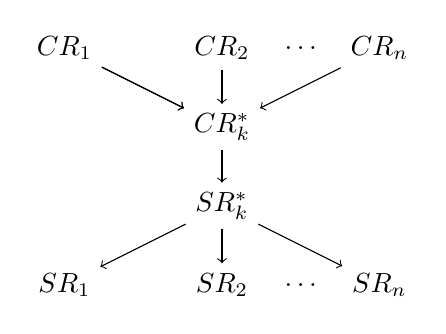
\begin{tikzpicture}
		
			\node (a) at (0,3)  {$CR_1$};
			\node (b) at (2,3)  {$CR_2$};
			\node (c) at (3,3)  {$\ldots$};
			\node (d) at (4,3)  {$CR_n$};
			
			\node (e) at (2,2)  {$CR_k^{*}$};
			
			\node (f) at (2,1)  {$SR_k^*$};
			
			\node (g) at (0,0)  {$SR_1$};
			\node (h) at (2,0)  {$SR_2$};
			\node (i) at (3,0)  {$\ldots$};
			\node (j) at (4,0)  {$SR_n$};
			
			\draw (a) edge[->] (e) 
			(a) edge[->] (e)
			(b) edge[->] (e)
			(d) edge[->] (e)
			(e) edge[->] (f)
			(f) edge[->] (g)
			(f) edge[->] (h)
			(f) edge[->] (j);
			
		\end{tikzpicture}
		
		\caption{Requirement graph structure}
		\label{fig:graph}
	\end{figure}	

	To model this relationship in the Emfatic metamodel, the \texttt{Requirement} superclass has multivalued references of type \texttt{Requirement}, for it's children and parents. The two references are opposites of each other, because two way navigation through the requirements graph is very important for the performance of the EOL operations in the EVL constraints and the model management operations.
	
	An alternative solution, that was considered, is to have the children and parent references in the subclasses as shown in \autoref{fig:alt-req}. This way system requirements are restricted to have only system requirements as children and customer requirements only customer requirements as parents, and no validation is required. However an opposite for \texttt{systemParents} has to be both \texttt{customerChildren} and \texttt{systemChildren}, which is not possible in Ecore and being able to navigate from children to parents as well as the other way around is very important for the model management tasks. So this solution was ultimately discounted.
	
	\begin{figure}[h!]
	\begin{framed}
	\centering
	\begin{lstlisting}
class CustomerRequirement extends Requirement{
  ref Requirement[*]#(customerParents & systemParents) customerChildren;
  ref CustomerRequirement[*]#customerChildren customerParents;
}
	
class SystemRequirement extends Requirement{
  ref SystemRequirement[*]#systemParents systemChildren;
  ref Requirement[*]#(customerChildren & systemChildren) systemParents;
}
	\end{lstlisting}
	
	\caption{Alternative implementation of requirements decomposition.}
	\label{fig:alt-req}
\end{framed}
	\end{figure}
	

	\subsection{Requirement Conflicts}
	Requirements can also be in conflict with each other, which means that only one of them can be completed. Conflicts can exist only between the same type of requirement - system requirements can be in conflict with system requirements only and customer requirements with customer requirements only. This constraint is directly enforced by the metamodel - the two different types of requirements have different types of references. Also because the conflict relationship is symmetric and navigation from both ends of the reference need to be possible, opposites have to be used. However, Ecore does not allow a reference to be it's own opposites \cite{selfopposite} (e.g. \texttt{ref CustomerRequirement[*]\#conflicts conflicts;}), so instead two references have to be used - \texttt{conflictsIncoming} and \texttt{conflictsOutgoing}.
	
	Additional constraints on conflicts arise from the nature of requirements decomposition and progress. They are enforced by the EVL constraints. It does not make sense for requirements to decompose into requirements, with which they are in conflict. Also the descendants of two conflicting requirements must be two disjoint sets, otherwise, one of the requirements would not be completable without it's conflicting requirement being completed, which is a contradiction. Finally, two conflicting requirements should not both have 100\% progress, because only one of them should be completed.
	
	\subsection{Requirement Progress} \label{sec:progress}
	All requirements have a progress field which should be set by the user, if the requirement doesn't have any children or is the average of its children's progress otherwise. A possible implementation of the progress attribute is to just leave it to the user to calculate the averages and check for this in the EVL validation. This is error prone and far from user friendly. 
	
	In order to automate calculation of progress, the java code of the generated GMF editor (see \autoref{sec:editor} for details) had to be modified. In particular the RequirementImpl.java class file, which defines the implementation of requirement entities. An \texttt{updateProgress} method is added to the class, which calculates the average progress of all child requirements and sets it as the current requirement's progress. This method is called by a custom notification listener (\texttt{Adapter}) defined in the constructor of \texttt{RequirementsImpl} class. The listener does two things: Whenever the progress field of the \texttt{RequirementImpl} object is set, the \texttt{updateProgress} method of all parents is called. And whenever a new child is added, the \texttt{updateProgress} method is called for the current \texttt{RequirementImpl} object. This implementation guarantees that whenever the progress of a leaf requirement is set in the editor, a chain reaction would cause all ancestors of the requirement to update their progress.

	An additional constraint for the progress attribute is that it must be a valid percentage. This is checked for in the EVL validation.
	
	\subsection{Team Members and Test-cases}
	According to the specification team members should have an assigned relationship with requirements and test-cases should have a verification relationship with system requirements. These two relationships are implemented as references of type \texttt{Requirement} for team-members and of type \texttt{SystemRequirement} for test-cases. 
	
	The definition of the decomposition relationship, established in \autoref{label}, means that leaf requirements in a graph, fully describe the whole graph. This means that progress only needs to be made on those requirements and verifying only them with test-cases would mean their ancestors are verified. For this reason, a choice was made to restrict test-cases to verify only leaf requirements and allow team members to be assigned only leaf requirements.  
	
	\subsection{Testing} \label{sec:tests}
	In order to test the abstract syntax and constraints, five simple test models were used. Each model tests a different aspect of the constraints:
	
	\begin{itemize}[noitemsep]
		\item 1.Y1403115 - Tests requirement decomposition (dependencies).
		\item 2.Y1403115 - Tests id's, requirement description length and progress.
		\item 3.Y1403115 - Tests requirement conflicts.
		\item 4.Y1403115 - Tests test-cases.
		\item 5.Y1403115 - Tests team members.
	\end{itemize}
	
	Each test model contains a correct graph of objects (whose names start with "Correct") and also several incorrect ones (whose names start with "Error"). Together all the models demonstrate all of the constraint failure cases. The example models were incrementally modified during development, as new issues arouse. 
	
	There is also an example model called example.Y1403115 which conforms to the abstract syntax and constraints and can be used to run the model management operations.
	
	\section{Editor} \label{sec:editor}
	%Explain the editor for your DSL, justify the decisions that you have made,
	%and briefly argue why your editor provides an appropriate notation for your DSL.
	
	\subsection{Description}
	The editor for the DSL is an Eugenia \cite{eugenia} generated GMF \cite{gmf} diagram editor. It uses a graph based diagram notation and it provides four types of nodes (objects) - \texttt{CustomerRequirements}, \texttt{SystemRequirements}, \texttt{TeamMembers} and \texttt{TestCases}. Each type of object has a different colour border in order to improve readability of models and avoid visual ambiguity. All attributes of each object are editable from the text fields in the diagram.
	
	Connections in the visual editor represent relationships between objects. They are all colour coded and use different line styles to improve readability.
	
	\subsection{Justification}
	The editor allows users to create and modify the fields of each type of the four main entities - system and customer requirements, test-cases and team members. All references between the entities can be modelled using connections. The colour coding of diagram elements, makes models clear and easier to understand.


	\section{Model Management Operations}
	%Explain the model management operations for
	%your DSL, justify the decisions that you have made, and briefly demonstrate that
	%the model management operations can be used to fulfill the model management
	%tasks described in Section 1.	
	
	\subsection{Model to Model Transformation}
	The M2M (Model to Model) transformation is implemented in the Epsilon Transformation Language (ETL) \cite{etl}, in a single ETL file. It takes an input model and creates an output model, removing all completed requirements. Following the ETL syntax, rules are defined for transforming each object in the input model to a equivalent object in the output model. The requirements transformation rule uses a guard in order to create requirements in the output model only if they are not completed in the input model. Also the children and parents for each requirement are filtered so that only non completed ones are created in the output model. Team members and test-cases are transformed only if they contain at least one non completed requirement. There are several abstract classes in the metamodel (see \autoref{sec:abstract}), so it makes sense to use ETL abstract transformation, in order to limit duplication.
	
	\subsubsection{Running Instructions}
	The M2M transformation can be ran using an ETL eclipse run configuration, which specifies an input model named "In" and an output model named "Out". The input model has to exist and be read on load.
	
	\subsection{Model to Text Transformation}
	The model to text transformation transformation (M2T) is implemented in the Epsilon Generation Language (EGL) \cite{egl} and is split across multiple EGL files:
	
	\begin{itemize}[noitemsep]	
		\item requirement2page.egl - Generates an html page from a requirement.
		\item teamMember2page.egl  - Generates an html page from a team member.
		\item testCase2page.egl - Generate an html page from a test-case
		\item model2index.egl - Generate main html page from requirementsModel.
		\item util.egl - Some utility functiions used to create links, lists of objects and nested list of requirements.
		\item main.egl - Coordinates the generation of all pages for a particular model. Uses input parameters so it can be reused for generating different versions of the same website.
		\item Y1403115.xml - ANT \cite{ant} build xml file, which generates a simplified model from the original one and then generates two versions of the website - one for the original and one for the simplified model and links them together.
	\end{itemize}

	The most complex requirement for the M2T transformation is the ability to filter out completed requirements. This is done by generating two versions of the website - one with all requirements and one with non completed requirements only. Every page of each version of the websites links to the main page of the other. In order to generate the simplified version of the website the M2M transformation described in the previous chapter is used. Chaining M2M and M2T transformations is a common model driven engineering pattern, which improves maintainability of the model management operations. Also the EVL validation is used to verify that the original model satisfies all constraints before the M2M transformation. At the end the ANT workflow consists of the following steps:
	
	\begin{enumerate}[noitemsep]
		\item Read original model.
		\item EVL validation on original model.
		\item M2M transformation of original model to simplified model.
		\item M2T transformation of original model.
		\item M2T transformation of simplified model.
	\end{enumerate}
	
	The main.egl, script uses input parameters suffix -  a string appended to the links of the current website version, otherSuffix - the suffix of the other website version and message - the text displayed in the link to the other website version. Each html page name in the website is formed by the id attribute of the object, the page is for, with the suffix appended. The main page file name in the website is \texttt{index + suffix + .html}.
	
	Instead of using an .egl file for the main transformation script, an .egx file could be used. This alternative was considered, however parameters could not be passed to the egx script. This meant that the .egx script could not be reused to generate two versions of the website and this is why this alternative was discounted.
	
	\subsubsection{Justification}
	Requirements/test-cases decomposition tree can be drilled down, by following links to child requirements and associated test-cases. 	The progress of each requirement is shown as a progress bar on its corresponding page. Requirements corresponding to each team member/test-case are displayed on the main page of the website. Completed requirements can be filtered via the link to the alternative simplified version of the website at the top of each page.
	
	\subsubsection{Running Instructions}
	The transformation can be ran from the Y1403115.xml ANT build script. The input model has to be specified manually in the script and defaults to the example.Y1403115 model (see \autoref{sec:tests}). The location of the EVL validation, M2M and M2T transformations is hard coded in the script. The output location for the website is called "gen" and is in the current directory of the ANT script. 
	
\printbibliography

\end{document}
